\section*{5.rész 3.Hőterjedés síkfalban}
\addcontentsline{toc}{section}{}


\begin{tabular}{ | p{2cm} | p{14cm} | } 
	\hline
	Név & Kovács Dániel \\ 
	\hline
	Szak &  Mechatronikai mérnöki alapszak\\
	\hline
	Félév & 2019/2020 II. (tavaszi) félév \\ 
	\hline
\end{tabular}
\vspace{0.5cm}

A hőterjedés síkfalban hővezetés formájában tud lezajlani. A hővezetés az energia térbeli terjedésének az a formája, amikor a hő egy közeg egyik − magasabb hőmérsékletű − részéből, annak másik része felé történő „áramlása” során a közeget alkotó részecskék elmozdulása nem számottevő, a részecskék rezgőmozgást végeznek.

Fourier törvénye szerint egy homogén testben a hőáram a csökkenő hőmérsékletek irányába mutat. Arányos a  hosszegységenkénti hőmérséklet-változással és a hőáram irányára merőleges keresztmetszettel. A megfigyelésen alapuló, hővezetésre felírt összefüggés:

\begin{equation*}
	 \dot{Q} = -\lambda A\frac{dT}{\delta}
\end{equation}

Ahol: \\
$\dot{Q}$ a hőáram, a felületen időegységenként átáramlott energia, $[\dot{Q}]$ = W \\
$\lambda$ a hővezetési tényező, az adott test anyagjellemzője, $[\lambda]$ = $\frac{W}{m K}$ \\
A a hővezető keresztmetszet, [A] = $m^2$ \\
$\frac{dT}{d\delta}$ pedig a hőmérséklet-eloszlás hely szerinti differenciálhányadosa, azaz a hosszegységenkénti hőmérséklet-változás, $[\frac{dT}{d\delta}]$ = $\frac{K}{m}$ \\

A hőáram és a keresztmetszet hányadosa - azaz a felület-egységenkénti hőáram - a hőáramsűrűség: $\dot{q}$ = $\frac{\dot{Q}}{A}$ , $[\dot{q}]$ = $\frac{W}{m^2 K}$ \\

Ezzel a Fourier-törvény: \\
\begin{equation*}
	 \dot{q} = -\lambda \frac{dT}{d\delta} = -\frac{\lambda}{d\delta} (T_2 - T_1) = \frac{\lambda}{\delta} (T_1 - T_2)
\end{equation}
\\
A Fourier-törvényben bevezetett hővezetési tényező $(\lambda)$ az anyag fizikai jellemzője, és azt fejezi ki, hogy mekkora a hőáramsűrűség 1 $\frac{K}{m}$ hosszegységenkénti hőmérséklet-változás esetén. A hővezetési tényező számértéke az adott anyag szerkezetétől és termodinamikai állapotától függ. Így a hővezetési feladatok egy részében, a testeken belüli hőmérséklet-különbségek nagysága miatt, a hővezetési tényezőt nem tekintjük állandónak. A gyakorlatban többnyire a hőmérséklettel való lineáris kapcsolatot feltételezve, a $\lambda(T)$ = $\lambda_0 (1 + bT)$ alakú összefüggés használata megfelelő pontosságú eredményt ad.


A Fourier-törvényt - figyelembe véve $\lambda$ hőmérséklettől való függését - így írhatjuk: \\
\begin{equation*}
	 \dot{q} = -\lambda(T) \frac{dT}{d\delta} = -\lambda_0 (1 + bT) \frac{dT}{d\delta}
\end{equation}
\\
A változók szétválasztása, és az egyenlet integrálása után az eredmény: \\
\begin{equation*}
	 \dot{q} = \frac{\lambda_0}{\delta} [(T_1 - T_2) + \frac{b}{2} (T_1^2 - T_2^2)]
\end{equation}
\\
amit ebben az alakban is írhatunk: \\
\begin{equation*}
	 \dot{q} = \frac{\lambda_0}{\delta} [1 + \frac{b}{2} (T_1 + T_2)] (T_1 - T_2) = \frac{1}{\delta} \lambda_a_t_l_a_g (T_1 - T_2) , \lambda_a_t_l_a_g = \lambda (\frac{T_1 + T_2}{2})
\end{equation}
\\
Azaz, a hővezetési tényezőt a középhőmérsékleten kiszámítva, a hőáramot az állandó $\lambda$ esetére érvényes összefüggésből kapjuk. \\
\\
\\
\\
\\
\\

Ábrázolhatjuk a hőmérséklet-hely függvényt, jelölve rajta a hőáram$(\dot{q})$ irányát
\\
\\

\begin{figure}[h]
	\centering
	\begin{subfigure}[b]{0.33\textwidth} 
		\centering
		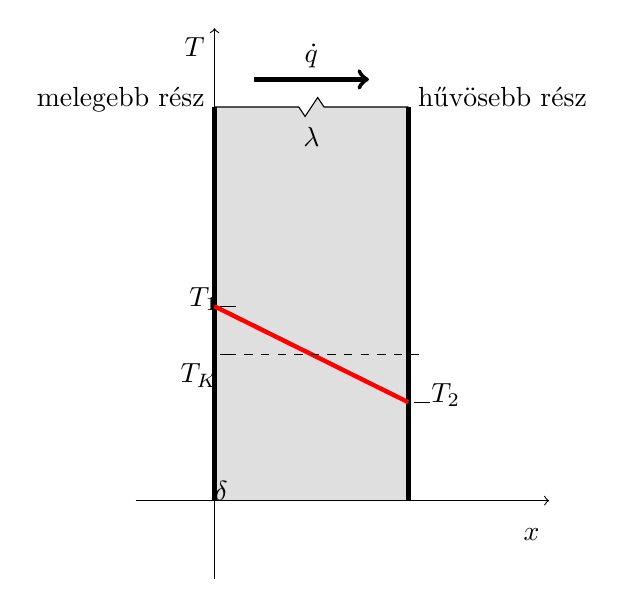
\begin{tikzpicture}
			\pgfmathsetmacro{\d}{16/6.5}
			\pgfmathsetmacro{\L}{5}
			\pgfmathsetmacro{\TA}{395/160}
			\pgfmathsetmacro{\TB}{200/160}
			\pgfmathsetmacro{\TK}{(\TA+\TB)/2}
			
			% Fal
			\fill[gray,opacity=0.25] (0,0) -- (0,\L) -- ({\d/2-0.16},\L) -- ({\d/2-0.08}, {\L-0.12}) -- ({\d/2+0.08}, {\L +0.12}) -- ({\d/2+0.16}, \L) -- (\d, \L) -- (\d, 0);
			\draw[] (0,\L) -- ({\d/2-0.16},\L) -- ({\d/2-0.08}, {\L-0.12}) -- ({\d/2+0.08}, {\L+0.12}) -- ({\d/2+0.16}, \L) -- (\d, \L);
			\draw[ultra thick] (0,0) -- (0,\L);
			\draw[ultra thick] (\d, 0) -- (\d, \L);
			
			% Feliratok
			\node[anchor=base east] at (0, \L) {melegebb rész};
			\node[anchor=base west] at (\d, \L) {hűvösebb rész};
			
			% Tengelyek
			\draw[->] (0,-1) -- (0,\L+1) node[anchor=north east]{$T$};
			\draw[->] (-1,0) -- (4.25,0) node[anchor=base east, shift={(0,-0.5)}]{$x$};
			
			% Hőáram és hőáramsűrűség
			\draw[->, ultra thick] (0.5,{\L+0.35}) -- ({\d/2},{\L+0.35}) node[anchor=south]{$\dot{q}$} -- ({\d - 0.5},{\L+0.35});
			
			% A hővezetési tényező
			\node[anchor=base] at ({\d/2},{\L-0.5}) {$\lambda$};
			
			% T(x)
			\draw[red, ultra thick] (0,\TA) -- (\d,\TB);
			
			% A delta_1 falvastagság
			\pgflength[xa=0, ya=0, xb=\d, yb=0, alim=0]{$\delta$};
			
			% A hőmérséklet értékek
			\draw (-0.1,\TA) -- (0.1,\TA);
			\node[anchor=base east] at (0,\TA) {$T_1$};
			
			\draw (-0.1+\d,\TB) -- (0.1+\d,\TB);
			\node[anchor=base west] at (\d,\TB) {$T_2$};
			
			% A közepes hőmérséklet
			\draw[dashed] (0,\TK) -- (\d,\TK);
			\draw (-0.1,\TK) -- (0.1,\TK);
			\node[anchor=north east] at (0,\TK) {$T_K$};
			
		\end{tikzpicture}
		\caption{A hőmérséklet-hely függvény}
	\end{subfigure}
\end{figure}
\pagebreak